\documentclass{bioinfo}
\usepackage{appendix}
\usepackage{multirow}
% \usepackage{algorithmic}
% \usepackage{fixltx2e}
% \usepackage{hyperref}
\copyrightyear{2010}
\pubyear{2010}

\begin{document}
\firstpage{1}

\newtheorem{theorem}{Theorem}[section]
\newtheorem{lemma}[theorem]{Lemma}
\newtheorem{proposition}[theorem]{Proposition}
\newtheorem{corollary}[theorem]{Corollary}

\newenvironment{definition}[1][Definition]{\begin{trivlist}
\item[\hskip \labelsep {\bfseries #1}]}{\end{trivlist}}
\newenvironment{example}[1][Example]{\begin{trivlist}
\item[\hskip \labelsep {\bfseries #1}]}{\end{trivlist}}
\newcommand{\todo}[1]{\textcolor{red}{#1}}
\def\INDC{{\bf 1}}
\newcommand{\update}[1]{\textcolor{blue}{#1}}
\newcommand{\old}[1]{\textcolor{green}{#1}}
\newenvironment{remark}[1][Remark]{\begin{trivlist}
\item[\hskip \labelsep {\bfseries #1}]}{\end{trivlist}}
\title[NETGEM]{NETGEM: Network Embedded analysis of Temporal Gene Expression Model}
%\title[short Title]{Analysis of temporal gene expression using mixture models}
\author[Sample \textit{et~al}]{Vinay Jethava$^{1}$, Chiranjib
  Bhattacharyya$^{1}$, Devdatt Dubhashi$^{2}$, Goutham N. 
Vemuri$^{3}$\footnote{to whom correspondence should be addressed}}
\address{$^{1}$Computer Science and Automation Department, Indian Institute of Science,
Bangalore, INDIA\\
$^{2}$Department of Computer Science, Chalmers University of
  Technology, G\"oteborg, SWEDEN\\
$^{3}$Systems Biology Division, Department of Chemical and Biological Engineering, Chalmers University of
Technology, G\"oteborg, SWEDEN\\
}

\history{Received on XXXXX; revised on XXXXX; accepted on XXXXX}
\editor{Associate Editor: XXXXXXX}

\maketitle

\begin{abstract}
\section{Motivation}
Temporal analysis of gene expression data has been limited to identifying genes whose expression varies with time and/or correlation between genes what have similar temporal profiles. Often, the methods do not consider the underlying network constraints that connect the genes. In addition to identifying changes in the genes, it is becoming increasingly evident that interactions change substantially. Thus far, there is no systematic method to relate the temporal changes in gene expression to the dynamics of interactions between them in the context of a regulatory network. The availability of this data opens up possibilities for discovering new mechanisms of regulation and provides valuable insight into identifying time-sensitive interactions. Furthermore, such a framework would also allow for studies on the effect of a genetic perturbation on the dynamics of the interactions.
\section{Results}
We present NETGEM, a tractable model rooted in Markov dynamics,
 for analyzing temporal profiles of genetic expressions arising 
out of known protein interaction networks evolving with unknown dynamics. 
The model treats the interaction strengths as random variables which
are modulated by suitable priors. This approach is necessitated by the
extremely small sample size of the available observations. The model
is amenable to a linear time algorithm for efficient inference. 
 When applied to real data
 NETGEM was successful in  identifying (i) temporal interactions and determining their strength, (ii) functional categories of the actively interacting partners and (iii) dynamics of interactions in perturbed networks. 
\section{Availability:}
The source code for NETGEM is available from http://www.sysbio.se/BioMet

\section{Contact:} goutham@chalmers.se 
\end{abstract}


\section{Introduction}
Gene expression microarrays are increasingly being used to determine transcriptional regulation  in response to a genetic or environmental perturbation. 
This has generated a vast amount of quantitative data which have compelled the use of statistical methods to identify differentially expressed genes and 
thereby, deduce transcriptional regulation. 
The general theme of these methods is to cluster genes, assuming that co-expressed genes are co-regulated. Often the inference is presented as a static network of genes that are activated or repressed by relevant transcription factors. 
This representation is similar to a wiring diagram of electrical circuits \citep{Stigler2007}. Important parameters of regulation such as amplitude of the 
signal, time lag, etc in such networks can only be studied by explicitly 
modelling the dynamics of such a system. This has spurred interest in 
analyzing time series gene expression data.

Conventional methods of time series analysis may not apply to this 
problem as the data has many interesting properties e.g.  observations close together in time are more closely related \citep{Glass1993}. The analysis is 
further complicated  by the fact that
 extremely small number of observations from different time points are available relative to variables (genes). 
There is the inherent risk of many genes having similar expression profile, just by random chance. Recognizing these problems, it is only recently that dedicated methods are being developed to infer temporal regulation of transcription \citep{Leek06EDGE, Ernst06STEM, Ramoni02cluster}, although temporal gene expression data are available much earlier. 
These, and other methods reviewed recently \citep{Androulakis2007} do not consider any dependency of observations between time points and hence are not suitable for the problem at hand.



Previous methods which have focused on identifying temporal changes in the genes and/or identifying correlations in their temporal expression profiles 
have ignored the dynamics of interactions between them. 
In recent work \citep{Song09KELLER}, time-sensitive interactions were identified based on local neighbourhood selection with $L1$-regularization to obtain sparse networks. The analysis learns the topology of the network from the data, and assumes a
smooth variation in the network interactions strengths to overcome the unreliability of results due to the small number of observations. 
This approach is extremely insightful in cases where the topology of the underlying network is unknown. 

However, when network structure is known, as in the case of regulatory
networks, there is an obvious benefit in incorporating this
information into analyzing the dynamics of the
interactions. Furthermore, it is of fundamental biological interest in
determining time-sensitive components of the networks. Currently there are no models which can be used for this purpose.

% In this paper, we consider the problem of learning a model from 
% temporal profiles of genetic expressions for a regulatory network 
% with a known structure.
% It is interesting to note that the dynamics has a direct bearing 
% on the profiles but it is unobserved, and stochastic 
% in nature.  This motivates a markovian approach for building such models.
% However inferring a general model of the time-varying interactions turns out
% to be an NP-hard problem. Learning of model parameters is further complicated by the
% small number of observation points.  

The interaction networks of baker's
yeast, {\it Saccharomyces cerevisiae} are arguably the most
well-constructed with a high level of confidence
\citep{Petranovic2009}. Therefore, we used this network 
to study and validate our models. 
The genes and proteins in yeast are classified according to their biological function \citep{Mewes2007} to a high degree of resolution. This allows the possibility to relate functional classification of the network components with the temporal interactions between them.

This line of argumentation leads to two very fundamental questions: (i) can we distill observations about temporal characteristics of a group of functionally similar genes? (ii) would it be possible to model the effect of a genetic perturbation (gene deletion or addition) while comparing temporal interactions between the reference strain and its perturbed mutant? 

In this paper, we introduce NETGEM, which stands for ``Network Embedded
  analysis of Temporal Gene Expression Model'',  a generative model for
temporal expression data which is capable of 
capturing the interaction dynamics in the network. Our approach
incorporates network effects into a basic underlying Markovian dynamics, and
also handles variation across closely related species.  A fundamental premise of
the model is that the evolution of the interaction strengths can be
modeled in terms of the functional categories of the interacting
genes. To the best of our knowledge, this is the first time such a
model has been investigated. Our case studies with synthetic and real
data show promising results. 


One could of course consider a simple Hidden Markov Model (HMM) for
modeling the interaction dynamics. Unfortunately, such a model becomes
intractable as the number of hidden states is exponential in the
number of interactions in the network. The problem of learning such a
model is further complicated by the small number of available
observation samples. NETGEM addresses this problem by assuming that
the interaction strengths evolve \emph{independently} of each other. 
This assumption leads to a model where one can derive efficient inference 
procedures which have linear time complexity 
in number of temporal observations. To handle the problem of low
sample size,  we adopt a Bayesian approach by introducing appropriate
priors over the parameters 
governing the evolution of the interactions.  Information from
multiple strains which are slight perturbations of a reference strain
are incorporated by effects determined by the underlying network. The
basic assumption is that interactions near the point of perturbation
(gene deletions) are affected more strongly than those far away from
the point of intervention. 

The remainder of this manuscript is organized as follows:
Section~\ref{sec:known-network} describes the construction of the
high confidence network. Section~\ref{sec:factorial-model} presents
the independently evolving weights assumption for tractable inference.
Section~\ref{sec:strain-damping-model} 
presents the variant for handling multiple strains.  
Section~\ref{sec:discussion-netgem} presents the main contribution of
the paper, i.e., the generative model NETGEM. We present the
experiments on synthetic and real datasets in
Section~\ref{sec:experiments} and conclude in Section~\ref{sec:conclusions}.


\begin{methods}
\section{Methods}
\label{sec:methods}
\subsection{Datasets and Interaction network}
\subsubsection{Gene expression Data}
\label{sec:gene-expression-data}
 Temporal gene expression datasets from {\it Saccharomyces cerevisiae} were downloaded from Gene
 Expression Omnibus using accession numbers XXXXX and GSE9644 . The two
 datasets were obtained using Affymetrix platform. The first dataset
 contained the expression profiles of the genes in {\it S. cerevisiae}
 during the gradual increment in the availability of glucose. Therefore, the cells experience a nutrient transition from glucose starvation 
 to nitrogen starvation. The transition was achieved by
 gradual increment of glucose availability in the feed to the cells,
 while keeping the nitrogen concentration constant in a D-stat
 \citep{Farzadfard2010}. The data was measured at eight time points. Beyond a certain concentration of glucose,
 nitrogen became the limiting nutrient. The cells underwent changes
 related to growth rate as well as metabolism. This dataset is referred to as EXP1 in this manuscript.
 Analysis of genes whose  expression significantly changed indicated that Sfp1 transcription
 factor played a dominant role in the bringing out the response to
 transition. In the interest of coherence, we chose a dataset that
 contains the temporal gene expression profiles in {\it sfp1} deletion
 mutant and its isogenic reference at different time points after
 pulsing steadily growing cells with glucose \citep{Cipollina2008}. The reference strain is referred to as REF, the strain in which {\it sfp1} was deleted is referred to as MUT. The data was measured at
 six time points after the pulse. This dataset is referred to as EXP2 in this manuscript. All raw data was normalized and preprocessed in R programming environment using BioConductor suite of tools \citep{Gentleman2004}.

\subsubsection{Construction of the interaction network}
\label{sec:known-network}
The yeast interaction network was constructed using previously published data~\citep{Gavin2002,Ho2002,Gavin2006,Krogan2006,Ito2001,Uetz2000} as well as 
data downloaded from BIND~\citep{Bader:2003:Nucleic-Acids-Res:12519993}, MIPS~\citep{MIPS},
MINT~\citep{citeulike:3733950}, DIP~\citep{citeulike:226627} and
BioGRID~\citep{citeulike:814974}. We used only those interactions that were backed by at least two independent sources, resulting in a high-confidence protein interaction network. 
We excluded protein-DNA interactions since the result of this interaction is the gene expression and including these interactions would result in a cyclic relationship between the interactions and gene expression. We overlaid the gene expression data onto the protein interaction network. 
Therefore, inherent in this is the assumption that gene expression is translated into protein abundance uniformly among all proteins.

\subsection{Model description}
This section presents the basic observation model which relates the
observed gene expression data to the high confidence interactions
network. We begin by defining the following notation, 
\subsubsection{Notation}
We assume that the base underlying network of interactions is known as a
graph $G=(V,E)$ as described in the previous section. Under different conditions, some of the edges are 
switched on or off, or, more generally set at various levels of
activation, $\mathcal W$. Also, the same edge may be active in one
strain and not in others at any given time point. Thus, we model the
state of the network by activation levels, $\mathbf{w}^{s}(t) = \{w^s_{e}(t)\}_{e
\in E}$, where $w^s_{e}(t)$ is the activation level of the edge $e$ at time $t$ in strain $s$. 

We use the notation $x^{s}_{e}(t)$ to denote the expression
levels for genes, $i$ and $j$, consisting the edge, $e=(i,j)\in E$,
for strain, $s$, at time $t$. Similarly,  $x_{e}^{1:S}(t_{a}:t_{b})$
denotes the observations for gene expression levels for edge,
$e=(i,j)$, over the set of strains, $\{1,\ldots, S\}$; for the time
interval, $\{t_{a}, (t_{a}+1), \ldots, t_{b}\}$. 

In the following sections, we will describe the building blocks
of our generative model, NETGEM. We begin by describing the overall
process dynamics as follows. 

\subsubsection{Observation model}
\label{observation-model}

The observed gene expression levels, $\mathbf{x}^{s}(t)$, for an strain
$s$ at time $t$ are modeled as an Ising system \citep{Song09KELLER}:
\begin{equation}
\label{eq:ising}
 P\left(\mathbf{x}^{s}(t) | \mathbf{w}^{s}(t)\right) = 
      \frac{1}{Z(t)} \exp \left( - \sum_{(i,j) \in E} w^s_{(i,j)}(t)
        x^{s}_i(t) x^{s}_j(t)\right)  
\end{equation}
where $Z(t)$ is the normalization constant. 

\subsubsection{Evolution model }
\label{sec:evolution-model}
We assume that the weights evolve according to the Markov chain, i.e.,
\begin{equation}
  \label{eq:q-evol}
 P(\mathbf{w}(t+1) = \mathbf{w}_{t+1} |  \mathbf{w}(t) = \mathbf{w}_{t}) = \mathbf{Q}(\mathbf{w}_{t}, \mathbf{w}_{t+1})
\end{equation}
where $\mathbf{Q}(\mathbf{w}_{t}, \mathbf{w}_{t+1})$ is the probability of the
transition from state $\mathbf{w}_{t}$ at time $t$ to state
$\mathbf{w}_{t+1}$ at time $(t+1)$. In general, if there are $S$
strains present, then each will have corresponding transition
probability matrix $\mathbf{Q}_{s}$. 

 
The problem, then, is to estimate the transition probability matrix for
strains, $\mathbf{Q}_{s}$, based on the observed gene expression values over
multiple strains, $\mathbf{x}^{1:S}(t)$, are the observed variables
and the strengths of the interaction network, $\mathbf{w}^{s}(t)$, is  the
hidden variable at time $t$. A direct HMM based approach requires $O({\mathcal W}^{2
  N_{e}}T)$ computations, where, ${\mathcal W}$ is the number of
possible discrete states for an edge activation strength, $N_{e}$ is
the total number of edges, and $T$ is the time 
period for which observations are made.  This is prohibitively
expensive for most practical problems. 

% The following section presents a practical scheme which solves the
% previous problem by  assuming that 
% the interaction strengths evolve independent of each other. 

\subsection{Independent weights dynamics}
\label{sec:factorial-model}
As noted in the previous section, applying the standard forward
backward algorithm is prohibitively expensive for moderate sized
graphs. So, we make the simplifying assumption that the weights are
evolving \emph{independent} of each other. This allows the
characterization of the overall probability distribution in terms of
the interaction strengths,  
\begin{eqnarray}
  \label{eq:q_mf}
  \hat{P}({\mathbf w}^{t}) &=& \prod_{e\in E} P_{e}(w_{e}^{t}) \\
  \hat{P}(w_{e}^{t+1} = w_{l} | w_{e}^{t} = w_{m}) &=& q_{e}(l, m) \label{eq:q-e-mf}
\end{eqnarray}

This allows us to model the evolution characteristics of each
interaction (edge) in the known network independently. Then, the
problem is the learning of the transition probability matrix for each
edge based on the observed gene expression levels. % We present
% theoritical justification for the assumption in
% \ref{sec:validity-assumption} and present experimental verification in section~\ref{sec:validation}.
% We employ a Bayesian
% approach~\citep{Gelman03bayesian,Beal03},  which have often been used to
% solve inference problem where there are few observation samples
% available, to solve the problem  of learning the transition
% probability matrices for each interaction (edge) in the known network.

% Figure~\ref{fig:factorial} shows the graphical model corresponding to
% the known network model with cluster similarity. We present a method
% of incorporating the information from multiple slightly perturbed
% strains into the inference algorithm in the following section. 
 

% $P(\mathbf{w}^{s}(t+1) = \mathbf{w}_{t+1} |  \mathbf{w}^{s}(t) =
%   \mathbf{w}_{t}, \mathbf{w}^{s}(t-1) = \mathbf{w}_{t-1},
%   \ldots) = P\left(\mathbf{w}^{s}(t+1) = \mathbf{w}_{t+1} |  \mathbf{w}^{s}(t) =
%   \mathbf{w}_{t}\right)$ for each strain. 
% We denote $Q$ as the
% transition probability of strain, $s$, such that
% \begin{equation}
%   \label{eq:Q-s}
%   Q^{s}(l, m) = P(\mathbf{w}^{s}(t+1) = \mathbf{w}_{m} |  \mathbf{w}^{s}(t) =
%   \mathbf{w}_{l})
% \end{equation}

\subsection{Analysis of Perturbed Networks}
\label{sec:strain-damping-model} 
We consider the problem of multiple strains which are just slightly
altered versions of the networks where a few genes have been knocked out of the
network. Therefore, most of the network remains the same across
strains with only the ``close'' neighbourhood of the knocked out genes
being affected. % Thus, if one looks at a ``far'' edge,
% $e_{far}$, the activation strength, $w_{e_{far}}(t)$, should be the
% same across strains  the gene expression data for the edge strains,
% $x^{1:S}_{e_{far}}(t)$, should be like i.i.d. samples, generated with
% the same activation strength, $w_{e_{far}}(t)$. In the following discussion, 
% we present a heuristic method which incorporates the ideas mentioned
% above into the inference problem. 
We assume that the weights corresponding to the reference strain
$\mathbf{w}(t)$ evolve according to a Markov law given by a matrix $Q$,
where $Q(l, m) = P(\mathbf{w}(t+1) = \mathbf{w}_{m} | {\mathbf w}(t)
= \mathbf{w}_{l})$ with the property that $\sum_{m} Q(l, m) = 1$ for
all the initial states $\mathbf{w}_{l}$. For other strains, we assume
that the corresponding values are just slightly perturbed; thus
\begin{equation}
  \label{eq:damping}
 w^s_e(t) = w_e(t) \Gamma^s_e
\end{equation}
The perturbing parameters $\Gamma^s_e$ are determined
deterministically from the underlying network $G$ by
\begin{equation}
  \label{eq:edge-damping}
\Gamma^s(i,j) = (1 - \gamma^s_i)(1 - \gamma^s_j)  
\end{equation}
where $\gamma^s_i \in [0,1]$ is a label determined by how far the gene
$i$ is in the underlying network to one of the genes knocked out in
strain $s$. We note that the deterministic nature of the damping
implies that all strains evolve similarly, i.e., $Q^{s} = Q\;
\forall \; s$. This allows us to incorporate the information for gene
expression levels in the different strains while learning the temporal
evolution characteristics. 

We compute the damping factor, $\gamma^s_i$, for the genes
as follows: If the gene, $i$, is knocked out in strain $s$, then we
label it as $\gamma^s_i=0$. Now, we diffuse the labels across the
graph  such that $\gamma^{s}_i = \frac{1}{d(i)} \beta
\sum_{j\in N(i)} \gamma_j^s$, i.e., the damping factor at a node is
the average of the damping factors at its neighbours.    

 Intuitively, while $\Gamma_e = 0$ for an edge 
directly incident to one of the knocked out genes, the perturbation
gradually damps out with distance from the knocked out gene and for
an edge $e$ far away from one of the knocked out genes, $\Gamma_e
\approx 1$.%  Sections~\ref{sec:validation} and
% \ref{sec:synthetic-dataset} present an experimental validation of the
% model.

% The next section extends the model by incorporating the functional
% hierachy of genes in the inference procedure. 

\subsection{Incorporating functional categories via mixtures}
\label{sec:mixture-model}
Since genes belong
  to multiple categories, a mixture model is a naturally suited model
  to handle the influence of multiple functional categories in the
  inference procedure. 

This allows us to explore  the relationship between functional
categories and the temporal evolution characteristics of the genes
which fall in the same functional category.

We now define the problem concretely. There are $H$ possible gene
categories. Each gene can be a member of one or more hierarchical
classes, $\mathcal{C}=\{C_{1},\ldots , C_{H}\}$, where the
hierarchical class $C_{h}$ is characterized by evolution matrix,
$Q_{h}$. The evolution probability matrix, $Q_{e}$, for each edge,
$e\in E$, is given as 
\begin{equation}
  \label{eq:q-mixture}
  Q_{e} = \sum_{h=1}^{H} \alpha_{e,h} Q_{h}
\end{equation}
where $\alpha_{e,h}$ denotes the influence of hierarchical class
$C_{h}$ in the edge, $e$, such that $\sum_{h} \alpha_{e, h} = 1$
for all edges $e \in E$. 


\subsubsection{Prior on transition probabilities,  $(\Theta)$} 
\label{sec:bayesian-approach}
The learning of the model parameter is significantly difficult when
there are few time points. To alleviate this, we propose a prior, $\Theta$, on
the transition probabilities, $Q_{h}$.  % Often, when a point estimate is required, the
% approach defines a suitable prior on the model parameter and performs
% MAP estimation. In our case, the model parameters are the transition
% probabilities,  $Q_{h}$, characterizing the temporal  evolution of the
% interaction strengths, $w_{e}(t)$, defined on the edge, $e\in E$, in
% the network. 
The individual rows, $\vec{q}_{l}$, of the transition
probability , $Q_{h}$, can be thought about as drawn from a multinomial
distribution. The Dirichlet distribution is the conjugate 
distribution~\citep{Gelman03bayesian}  of the multinomial distribution
and hence naturally suited as a prior distribution. We model the
transition probabilities matrices as Dirichlet distributions, 
such that  the prior on the transition probabilities matrix, $Q$, 
given the parameter, $\Theta$, is
\begin{eqnarray}
  \label{eq:q_prior}
  P(\vec{q}_{l} | \vec{\theta}_{l}) &\sim& Dir(q_{l1}, \ldots, q_{l\mathcal{W}} ;
  \theta_{l1},\ldots, \theta_{l\mathcal{W}}) \\
&=& \frac{1}{B(\vec{\theta}_{l})} \prod_{m=1}^{\mathcal{W}} q_{lm}^{\theta_{lm}-1}
\end{eqnarray}
where $\vec{\theta}_{l}=[\theta_{l1},\ldots,\theta_{l\mathcal{W}}]$ and
$B(\vec{\theta}_{l})$ is the multinomial beta
function~\citep{Gelman03bayesian}.


\subsubsection{Choice of prior parameters $(\Lambda)$}
\label{sec:choice-prior-param}
We incorporate the effect of the functional classification of
genes on the mixture components,
$\vec{\alpha}_e$, for an edge, $e$, by using a Dirichlet prior of the form:
\begin{eqnarray}
  \label{eq:hier-prior}
  P(\vec{\alpha}_e) &\sim& Dir(\alpha_{e,1},\ldots, \alpha_{e,H};
  \lambda_{e,1},\ldots, \lambda_{e,H}) 
\end{eqnarray}
with the prior parameter, $\lambda_{e,h}$, for the edge, $e=(i,j)$, of the
form 
\begin{equation}
  \label{eq:mixture-prior}
  \lambda_{e,h} = \Big\{ \begin{array}{ll}
                       \lambda_p & \textrm{if genes }  i \textrm{ or } j
                       \textrm{ in class } h \\
                       \lambda_o & \textrm{otherwise}
                       \end{array}
\end{equation}

% Joint estimation of the parameters $\alpha_{e,h}$ and  $Q_{h}$ is
% not possible due to the dependence relationship given in
% (\ref{eq:q-mixture})~\citep{Dempster77em}.We use a standard technique and define the random variable
% $\mathbf{y}^{1:T} = \{y_e^t\}$ for all edges, $e \in E$,  and times,
% $t=\{1,\ldots, T\}$ where $y^t_e$ denotes the component from which
\subsubsection{Functional Category $(Y)$}   We define the random
variable $Y_{e}(t)$ which denotes the functional category 
chosen at time $t$ for edge $e$; such that the event $Y_e^t = h$
implies that $P(w_e^{t+1}= w_m | w^t_e =w_l, y_e^t = h) = q_h(l,
m)$. 
% This allows us to decouple the two estimation of $\alpha_{e,h}$
% and $Q_{h}$. 

\subsection{NETGEM: a generative model}
\label{sec:discussion-netgem}
\begin{figure}[htp]
  \centering
  \fbox{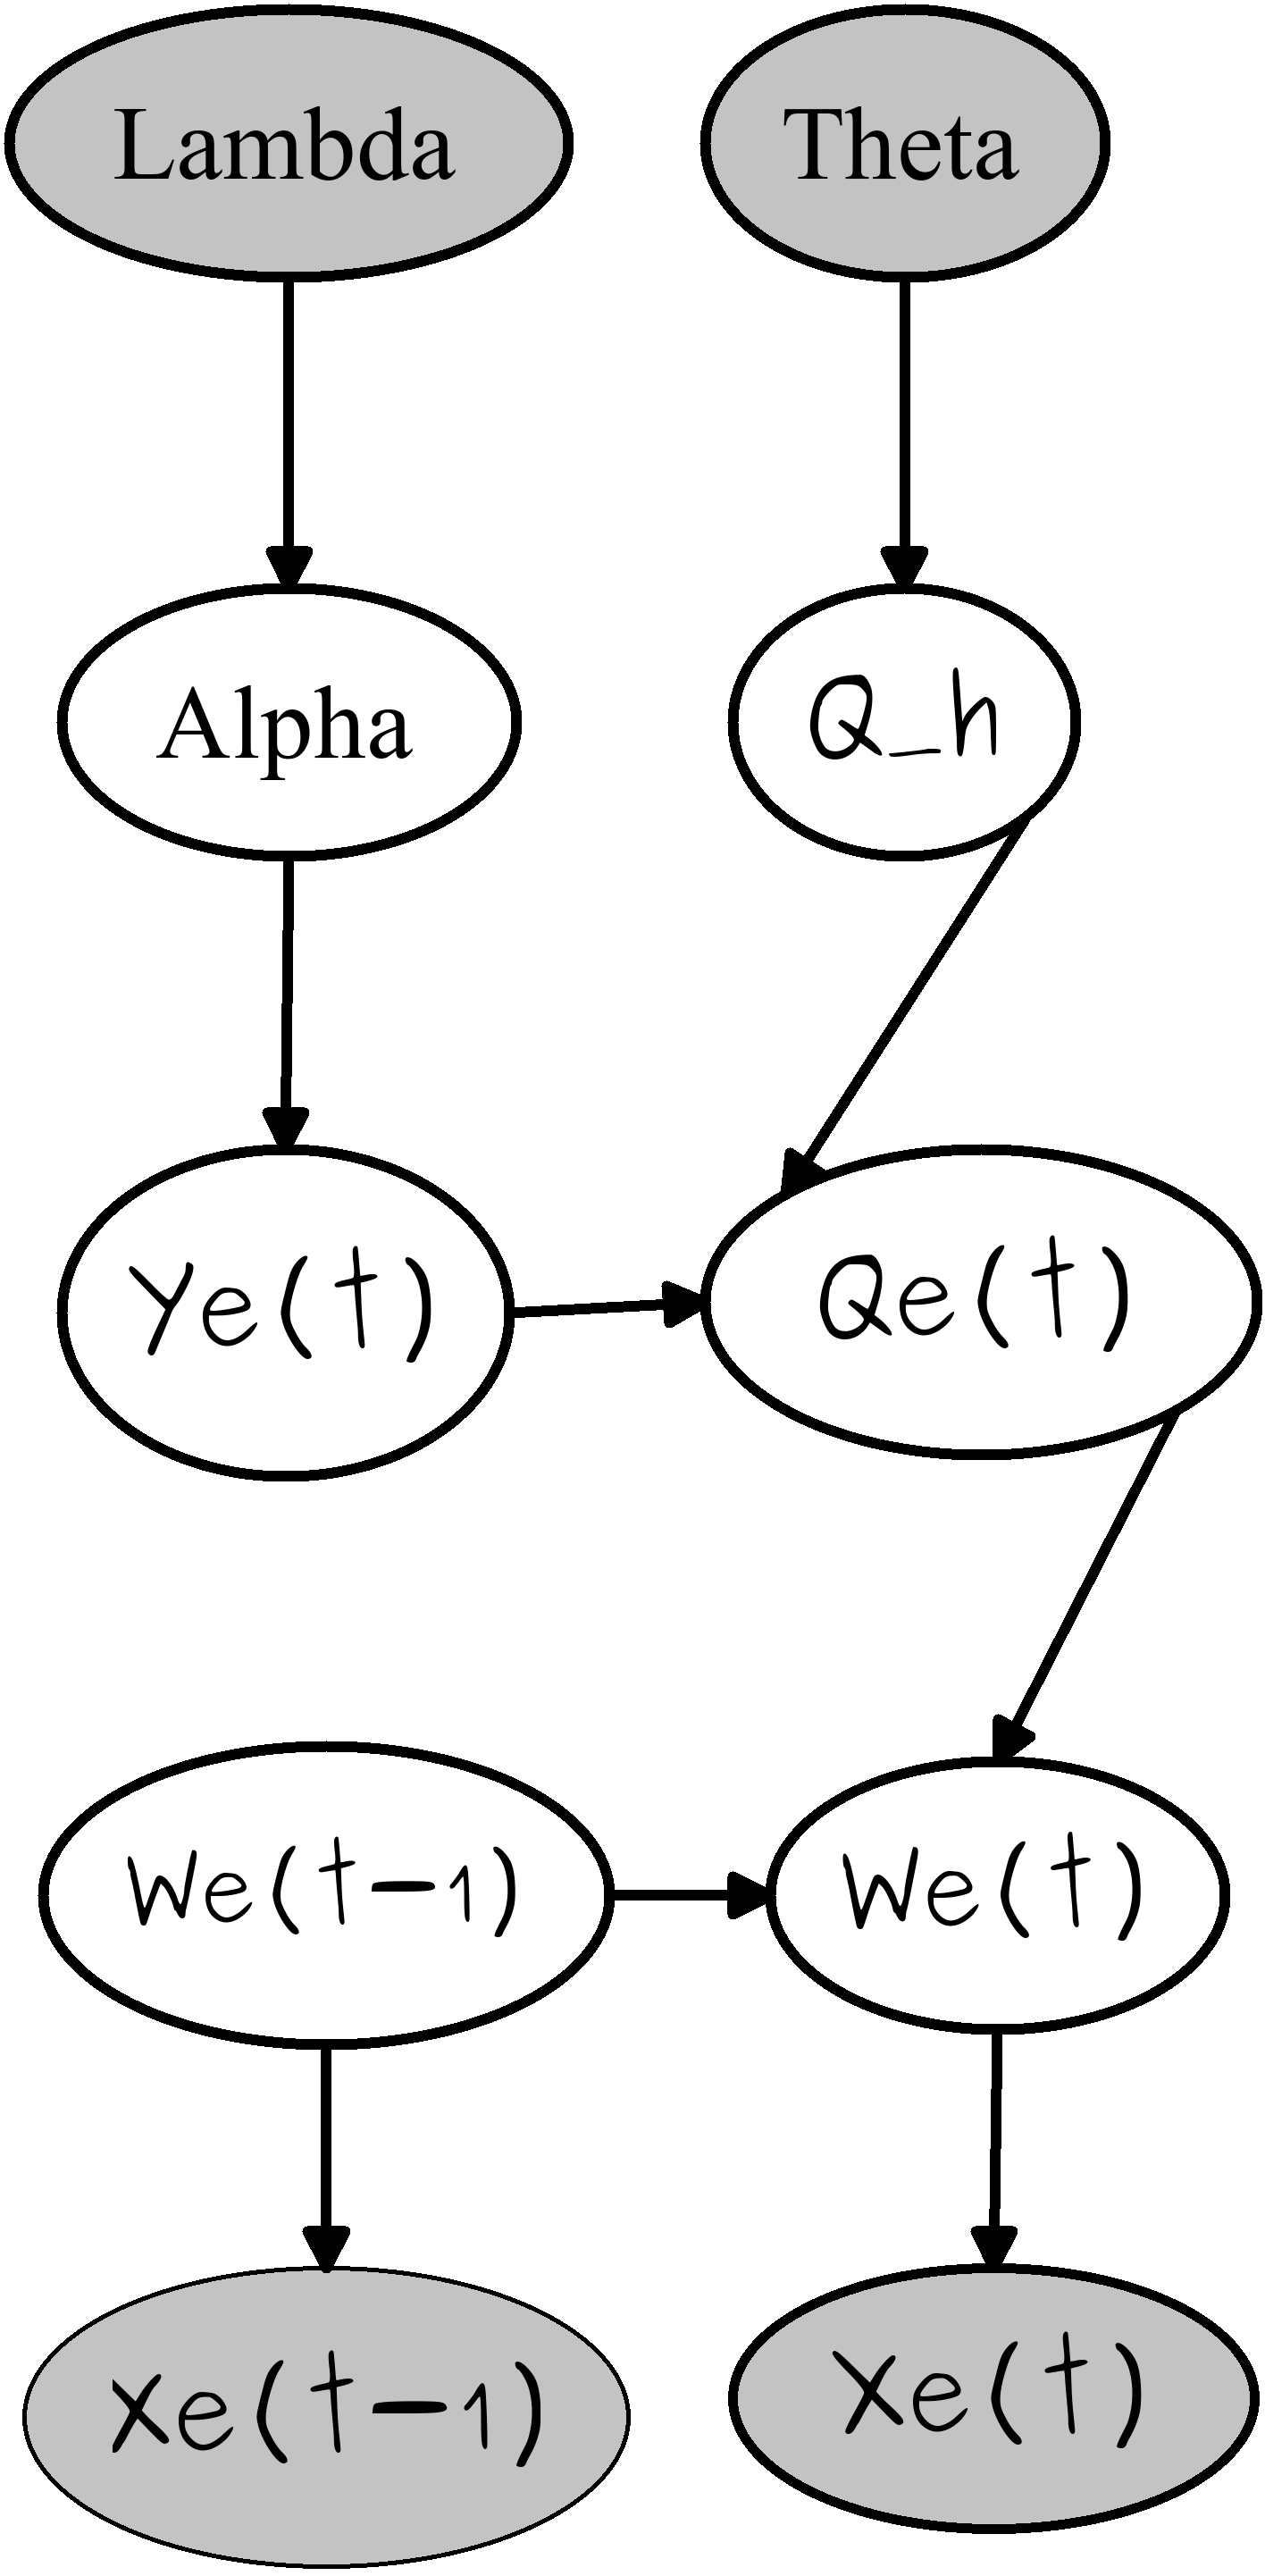
\includegraphics[scale=0.075,angle=90]{images/netgem}}
  \caption{Graphical model corresponding to the NETGEM generative
    model. The shaded nodes are known/observed. The inference is done
    over the hidden variables $\Omega = \{y_{e}(t), w_{e}(t)\}$; and the parameters to be learnt
    are $\Psi = \{Q_{h}, \alpha_{e,h}\}$ }
  \label{fig:netgem}
\end{figure}

We now present a unifying view of the NETGEM model as a generative
probabilistic model for gene expression data,
${\mathbf X}^{1:S}(1:T)$, for multiple strains $\{1,\ldots,S\}$ and
observation time points $\{1, \ldots, T\}$.  The quantities known
apriori are the number of classes, $H$; the set of edges, $E$; the
number of strains, $S$, and the number of observation points $T$. 

Figure~\ref{fig:netgem} shows the graphical model corresponding to the
NETGEM model. The inference is done over the hidden variables $\Omega
= \{y_{e}(t), w_{e}(t)\}$; and the parameters to be learnt are $\Psi = \{Q_{h}, \alpha_{e,h}\}$.

In addition, the hyper-parameters, $\Theta$ and $\Lambda$ need to be
specified which are described in Sections~\ref{sec:bayesian-approach}
and \ref{sec:choice-prior-param} respectively. Then, NETGEM models the
following generative process:
% \fbox{
\begin{enumerate}
\item Initialization 
  \begin{enumerate}
  \item For each functional category $h \in H$; Choose $Q_{h} | \Theta$,  s.t. each row, $\vec{q}_{i} \sim   Dir(\vec{\theta}_{i})$ 
  \item For each edge $e\in E$;  Choose mixture components, $\alpha | \Lambda$ s.t. $\vec{\alpha}_{e} \sim Dir(\vec{\lambda}_{e})$
  \end{enumerate}
\item For each time, $t \in \{1,\ldots, T\}$
  \begin{enumerate}
  \item For each edge $e \in E$
  \begin{enumerate}
  \item Choose $Y_{e}(t) \sim P(Y_{e}(t) = h) = \alpha_{e,h}$, The
    choice of $Y_{e}(t)$ fixes $Q_{e}(t)$ as $Q_{e}(t) | \{Y_{e}(t) = h\}  = Q_{h}$
  \item Choose $w_{e}(t) \sim P(w_{e}(t) | w_{e}(t-1), Q_{e}(t-1))$ as
    in (\ref{eq:q-e-mf})
  \item Compute $w_{e}^{s}(t) = \Gamma^{s}_{e} w_{e}(t)$
  \end{enumerate}
    \item Choose $X^{s}(t) | W^{s}(t) $ as in (\ref{eq:ising})
 \end{enumerate} 
\end{enumerate}
% }
The key principle underlying the model is that the interaction dynamics are
governed by the functional categories. In particular, for each edge $e$ and time
$t$, we generate a functional category, $Y_{e}(t)$. This functional
category is \emph{solely} responsible for the change of interaction strength
from $w_{e}(t)$ to $w_{e}(t+1)$. The interaction strengths affect the
observed gene expression data, through the strain damping model and
the Ising probability distribution~(\ref{eq:ising}). On the whole, this is equivalent to a
mixture of the corresponding functional categories with appropriate
mixing proportions. 

We now outline the expectation maximization procedure~\citep{Dempster77em} which
iteratively learns the unknown quantity, $\Psi = \{Q_{h},
\alpha_{e,h}\}$, for $h \in {\mathcal H} = \{1,\ldots, H\}$ and $e \in
E$ where  $Q_{h}$ is the class evolution
probability matrix for class, $C_h$, and $\alpha_{e,h}$ is the mixing
proportion for  edge, $e$ and class $C_h$; and $\Omega =
\{\mathbf{y}^{1:T},\mathbf{w}^{1:T}\}$ is
the hidden variable.  Let $\Psi^{(n)} = \{\alpha^{(n)}_{e,h},
Q^{(n)}_h\}$ be the estimates at the $n^{th}$ iteration. Then, 
\begin{equation}
  \label{eq:q-edge-mixture-em}
  \begin{array}[h]{llll}
  \textrm{E-step:} & {\mathcal L}(\Psi; \Psi^{(n)}) &=&
  E_{\Omega^{|} }  [ \ln P(\mathbf{x}^{1:S}(1:T), \Omega({1:T}) | \Psi({1:T}))] \\
\vspace{2 mm}
  \textrm{M-step:} & \hat{\Psi}^{(n+1)} &=& \arg\max_{\Psi} (\ln P(\Psi) +
  {\mathcal L}(\Psi; \Psi^{(n)} ) ) 
  \end{array}
\end{equation}
where $\Omega^{|}$ is the conditioned variable $(\mathbf{w}^{1:T},
\mathbf{y}^{1:T} | \mathbf{x}^{1:S}(1:T),  \Psi^{(n)})$.

The maximization step in (\ref{eq:q-edge-mixture-em}) can  be done
separately for $q_h(l,m)$ and $\alpha_{e,h'}$ independently. We use
the priors in (\ref{eq:q_prior}) and
(\ref{eq:hier-prior})-(\ref{eq:mixture-prior}), and the constraints
\begin{eqnarray}
  \label{eq:mixture-q-constraint-0} \sum_{m} q_h(l,m) &=& 1 \quad\forall h \\
   \label{eq:mixture-alpha-constraint-0} \sum_{h} \alpha_{e,h} &=& 1 \quad\forall e
\end{eqnarray}
to obtain the following update equations:
\begin{eqnarray}
  \label{eq:mixture-alpha-update}
  \alpha_{e,h'}^{(n+1)} =&  \frac{(\lambda_{e,h'}-1) + \sum_{t=1}^{T-1} \sum_{l,m,h}\xi^{t}_{e}(l,
    m,h,h') }{\sum_{h'} (\lambda_{e,h'} -1) + \sum^{T-1}_{t=1}
    \sum_{l,m,h,h'} \xi^{t}_{e}(l,m,h,h')} & \\
\label{eq:mixture-q-update} 
q^{(n+1)}_h(l,m) =&  \frac{(\theta_{lm}-1) + \sum_e \sum_{t=1}^{T-1}\sum_{h'}\xi^{t}_{e}(l,
    m,h,h') }{\sum_{m} (\theta_{lm} -1) + \sum_e \sum^{T-1}_{t=1}
    \sum_{m,h'} \xi^{t}_{e}(l,m,h,h')} &
\end{eqnarray}
where $\xi^{t}_{e}(l,m,h,h')$ is defined in
appendix~$1$.% \ref{sec:mixt-model-deriv}.

\subsubsection{Simplification: Independent weights dynamics model}
\label{sec:relat-indep-weights}
We now consider the simplification that each edge has its own
evolution characterization. In other words, suppose there are $H=E$
functional classes with corresponding priors $\Lambda$ defined such
that each row $\vec{\lambda}_{e}$ corresponding to edge $e$ has only
one zero entry. The inference in such a model is considerably simpler
since there is no learning of mixture components, $\alpha_{e,h}$. 

We call this model the independent weights dynamic, (IWD), model and
present the derivation for the inference and parameter learning in
appendix~$2$. %\ref{sec:fact-model-deriv}.

\subsubsection{Relation to the multiple strains}
The multiple strains in section \ref{sec:strain-damping-model} effect the probability $P(X^{s} | W^{0})$. If the strains are all identical (Section~\ref{sec:factorial-model}),
then, the observations $x^{s}_{i}(t)$ can be considered as
i.i.d. samples, i.e., the damping factor $\Gamma^{s}(i,j) = 1$ for all
$i, j$. 

\end{methods}

\section{Implementation}
\label{sec:experiments}
We present the experiments performed on synthetic and actual datasets
in this section. We compare the factorial weights and the mixture
model against a standard implementation of HMM which learn
the evolution characteristic for the system jointly in
\ref{sec:validation}. We present the results on two genetic
expressions datasets in~\ref{sec:real-world-datasets}.
  
\subsection{Validation of the models on synthetic datasets}
\label{sec:validation}

We consider a model, $M$, which provides estimates $\{\hat{\mathbf Q}^{M}\}$ and
  $\{\hat{{\mathbf w}}_{e}^{M}(t)\}$  for the true transition probabilities
  $\mathbf{Q} $ and the actual interaction strengths $\{w_{e}(t)\}$ for the
  edges $e\in E$ for the time period $t \in T$. Then, a standard
  hidden Markov model attempts to estimate $\hat{\mathbf Q}^{HMM}$
  directly. Our methods, respectively, the independent weights dynamics (IWE)
  model and the generative model (NETGEM), estimate the transition
  probabilities, $\hat{Q}_{e}$ defined over the edges $e\in E$ and
  then construct a rank-1 approximation, $\hat{\mathbf Q}^{IWE}$ and
  $\hat{\mathbf Q}^{NETGEM}$\footnote{Supplemental material}.

We choose a synthetic graph with $N=5$ nodes (genes) and $H=10$ functional
classes. The small value of $N$ allows direct estimation of the
transition probability matrix, $\hat{\mathbf Q}^{HMM}$,  of size ${\mathcal W}^{N} \times {\mathcal W}^{N}$,
using an standard implementation of HMM. %\footnote{http://people.cs.ubc.ca/~murphyk/Software/HMM/hmm.html}.
The genes are randomly assigned classes  such that each
node is a member of $N_{av}=1.5$ classes on average. The weights take
possible values in ${\mathcal W} = \{-1, 1\}$, and the evolution characteristic, $Q_{e}$ for
each weight is a mixture based on the interacting genes.  We compare
our the quality of the results obtained by our models against the
results obtained by the HMM for $N=20$ random trials. 


We use two metrics to compare our results with respect to the standard
hidden Markov model implementation over the large state space, namely, 
\begin{enumerate}
\item \emph{F1-score:} F1-score is the harmonic mean of the precision, $P$,
   and recall, $R$ , i.e., $F1 =\frac{2 P R}{(P + R)}$
    . In the context of our problem, the precision, $P_{M}$, and
  recall, $R_{M}$,  for a model, $M$, are defined as
  \begin{eqnarray}
    \label{eq:f-score}
    P_{M} &=& \frac{\sum_{e
  \in E} \sum_{t=1}^{T} \INDC_{\hat{w}^{M}_{e}(t) = 1 } \INDC_{w_{e}(t) = 1 } } {\sum_{e
  \in E} \sum_{t=1}^{T} \INDC_{w_{e}(t) = 1 }} \\
R_{M} &=&  \frac{\sum_{e
  \in E} \sum_{t=1}^{T} \INDC_{\hat{w}^{M}_{e}(t) = 1 } \INDC_{w_{e}(t) = 1 } } {\sum_{e
  \in E} \sum_{t=1}^{T} \INDC_{\hat{w}^{M}_{e}(t) = 1 }}
  \end{eqnarray}
 where $\INDC_{\{\cdot\}}$ is the indicator function. Thus, F-score measures the accuracy of the predictions about strengths of
 interactions made by the model.
\item \emph{Frobenius norm:} We measure the Frobenius norm between the
  estimated (by model $M$) transition probability, $\hat{\mathbf
    Q}^{M}$ and the true transition probability, $\mathbf Q$ used to
  generate the data, as
  \begin{equation}
    \label{eq:f-norm}
    || \hat{\mathbf Q}^{M} - {\mathbf Q} ||_{F} = \sum_{i, j} |q_{ij}^{M} - q_{ij}|^{2}
  \end{equation}
 where $q_{ij}$ denotes the $(i,j)^{th}$ element of the matrix
 $\mathbf Q$. Thus, this measures the accuracy with which we can estimate the
 transition probability, $Q$. 
\end{enumerate}

\begin{figure}[htp]
  \centering
  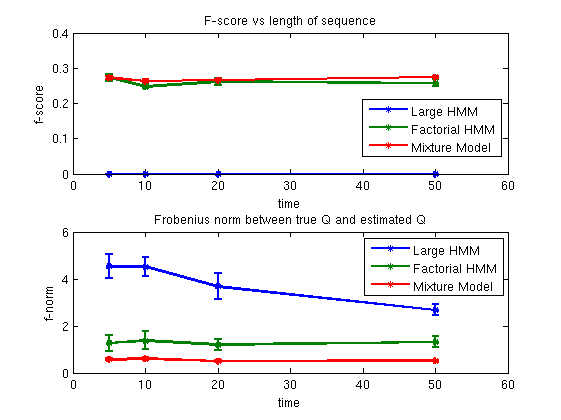
\includegraphics[scale=0.55]{results/mm_tvar}
  \caption{This figure compare the results obtained using the Independent weights dynamics model (IWE)
    and the generative model (NETGEM) with result of an standard HMM  implementation with
    increasing number of observations (time points), $T$,
    available for $20$ random trials. The colors denote HMM (blue), IWE (green),
    NETGEM (red)   (a) F-score for the estimated weight evolution {\it versus} the true
    weight evolution sequence (b) Frobenius norm of the difference between the true
    evolution characteristics for the system and the estimated characteristics. }
  \label{fig:validation-t}
\end{figure}
\begin{figure}[h]
  \centering
  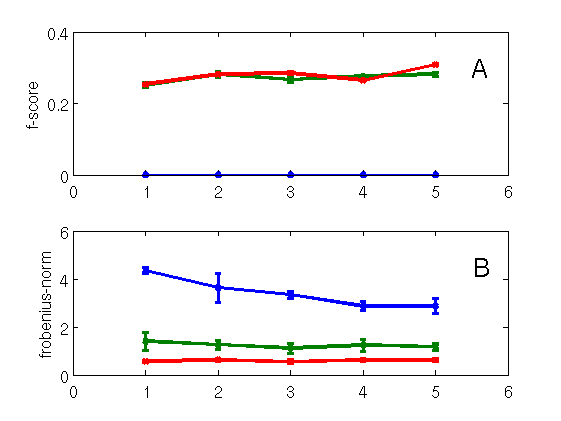
\includegraphics[scale=0.55]{results/mm_strain}
  \caption{This figure compare the results obtained using the Independent weights dynamics model (IWE)
    and the Mixture Model (NETGEM) with result of an standard HMM  implementation with
    increasing number of strains, $S$, available for $20$ random trials. The colors denote  HMM (blue), IWD (green),
    NETGEM (red). (a) F-score for the estimated weight evolution vs the true
    weight evolution sequence (b)
    Frobenius norm of the difference between the true evolution
    characteristics for the system and the estimated characteristics. } 
  \label{fig:validation-s}
\end{figure}


Figure~\ref{fig:validation-t} shows the comparison between different
methods with increasing length of the sequence, $T$. The results indicate that the
standard HMM requires longer sequences to get comparable results with
the IWD and NETGEM approach. 

Figure~\ref{fig:validation-s} compares the
methods with increasing number of strains present (with at most 1 gene
knocked out). We note that the performance of the models improves
slightly with additional number of strains. 

\subsection{Inferring interaction dynamics from gene expression data}
\label{sec:real-world-datasets}
This section  presents the experiments on real genetic expression
datasets. We begin by describing a procedure for identifying the interactions
which show a high degree of temporal variation in their strengths.  

\subsubsection{Identifying time-sensitive interactions}
\label{sec:ident-crit-inter}
 We apply our algorithm to infer the interaction strengths for two
genetic network scenarios. We are interested in the edges which show
considerable change during the measured time points. Towards this end,
we compute the change score, $s(e)$, of an interaction strength $w_{e}(1:T)$ as follows
\begin{equation}
  \label{eq:change-score}
  s(e) = \frac{1}{T} \sum_{t=1}^{T-1} (w_{e}(t+1) - w_{e}(t))^{2} 
\end{equation}
We fit an exponential distribution to it and consider the weights
falling in the top-$5 \%$ ($p=0.05$) tail of the
distribution. The interaction between the nodes was visualized as a
graph in the Cytoscape environment~\citep{Shannon2003}.

\subsubsection{Interaction dynamics in response to nutrient availability (Experiment 1):}
\label{sec:experiment-1}
The data in this experiment captures the changes in gene expression
during the gradual transition from glucose to ammonia as the
growth-limiting nutrient. Genes that have already been grouped into
eight clusters \citep{Farzadfard2010} were connected according to the
protein interaction network and the interaction strength between them
determined from gene expression using the model
(Figure~\ref{fig:exp-1-time-evol}).  The data in this experiment
captures the changes in gene expression during the gradual transition
from glucose to ammonia as the growth-limiting nutrient. Genes that
have already been grouped into eight clusters \citep{Farzadfard2010}
were connected according to the protein interaction network and the
interaction strength between them determined from gene expression
using the model. At the beginning of the experiment (t = 0), the cells
were starved for glucose and were progressively exposed to increased
glucose availability. After time t = 9.6, ammonia became the limiting
nutrient. Subsequent time points capture the changes that occur in the
presence of excess glucose. In response to this transition, we
observed corresponding changes in glucose and ammonia metabolism,
which are reflected in the interactions between the genes responsible
for the synthesis of proteins and lipids. For example, we observed a
strong positive (inductive) interaction between the genes of
carbohydrate metabolism and protein synthesis (top left corner of the
network) during glucose starvation. The interaction strength gradually
decreased until t = 9.6 hours and subsequently turned negative
(repressive). Since the genes in this cluster predominantly belong to
amino acid synthesis, our results indicate a gradual repression in
amino acid and protein synthesis upon the onset of ammonia starvation.

The transition in the growth-limiting nutrient also brought about an
abrupt change in the interactions between genes responsible for
ribosome biosynthesis (cluster of genes on the extreme right of each
network). Our model identified a momentary repression in the synthesis
of ribosomes at t = 9.6 hours, when the growth limitation was exerted
by ammonia. These genes were constitutively active during all other
time points, as is expected because ribosome biosynthesis is an
essential cellular process. The temporary arrest in ribosome
biosynthesis was attributed to the control exerted by Sfp1
transcription factor \citep{Farzadfard2010}. Our model also identified
positive interactions between amino acid metabolism and cell cycle and
negative interactions between genes of storage carbohydrates and lipid
metabolism (Figure~\ref{fig:exp-1-time-evol}). These interactions are
available as supplementary files. 


\begin{figure*}[htp]
  \centering
  \begin{tabular}{cccc}
  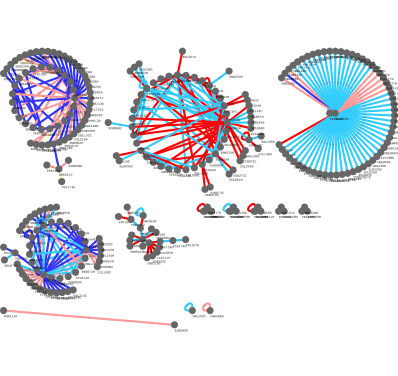
\includegraphics[scale=0.3]{results/aejoint/t1.png}
  &   
\includegraphics[scale=0.3]{results/aejoint/t2.png}
  &   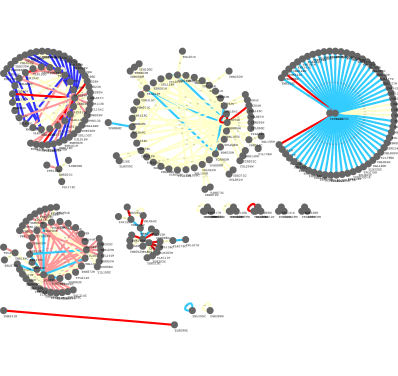
\includegraphics[scale=0.3]{results/aejoint/t3.png}
  &   
\includegraphics[scale=0.3]{results/aejoint/t4.png}  \\
   t=0.0 & t=4.1 & t=6.8 & t=9.6 \\ 
  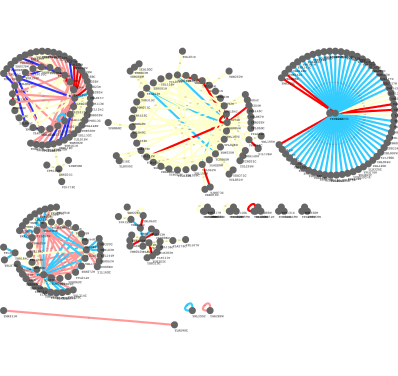
\includegraphics[scale=0.3]{results/aejoint/t5.png}
  &   
\includegraphics[scale=0.3]{results/aejoint/t6.png}
  &   
\includegraphics[scale=0.3]{results/aejoint/t7.png}
  &   
\includegraphics[scale=0.3]{results/aejoint/t8.png}  \\
  t=14.5 & t=27.3 & t=42.7 & t=53.9 \\ 
  \end{tabular}
  \caption{Time varying interaction strengths between the genes from Experiment 1. Each network is composed of all the genes from the eight clusters previously identified \citep{Farzadfard2010}, and is shown for the eight time points for which gene expression was measured. The time stamps (in hours) are indicated below each network. 
The edge colors denote their interaction strength, which was classified as strong repressing (red), low repressing (pink), no effect (yellow), low inducing (light blue) and strong inducing (dark blue).}
  \label{fig:exp-1-time-evol}
\end{figure*}
 
\subsubsection{Interaction dynamics in response to network perturbation (Experiment 2):}
\label{sec:experiment-2}
In order to test the utility of incorporating the damping our model in
capturing the impact of perturbations in the network, we used the
dataset in which the key transcription factor Sfp1 was deleted
\citep{Cipollina2008}. We chose this dataset since Sfp1 was previously
identified to be one of the most important transcription factors that
governed the response to nutrient availability in yeast
\citep{Farzadfard2010}. We first identified the interactions that are
sensitive to time and perturbation, as described in
\ref{sec:ident-crit-inter}. 
The histogram of the number of
edges was fit to an exponential distribution
(Figure~\ref{fig:hist-score}) and only those interactions that passed
the threshold cutoff of $p <= 0.05$ were considered for
subsequent analysis. In this manner, we identified 171 interactions
among the genes that were already identified to have differentially
expressed between REF and MUT (see
section~\ref{sec:gene-expression-data} for strain nomenclature). An
important aspect of novelty in our model is the incorporation of the
damping effect in the model. This model ensures that interactions
further from the point of perturbation in the network are affected to
a lesser degree than those closer to it. The effect of damping is very
sensitive to the network and in the network we considered in this
study, a majority of the edges appear to be relatively unaffected by
the perturbation (Figure~6).


After assessing the effect of perturbation for our network, we
identified temporal changes in the interactions in the REF strain as
well as the MUT strain independently (Figure~6). We observed
some overlap in the actively interacting genes between REF and
MUT. Many of these genes were hexose transporters and those
responsible for pH homeostasis. The genes (and the functional
categories) that are common to the strain indicate that they are not
responsive to the mutations. The utility of NETGEM in identifying the
temporal interactions that are different between REF and MUT is
indicated by the identification of many genes that are responsible for
ribosome biosynthesis and amino acid metabolism (Figure~6). The results concur with the known role of Sfp1 in
coordinating metabolism with ribosome biosynthesis. These interactions
were identified by considering gene expression profiles in REF and
MUT, using the damping model. Indeed the functional classification of
the genes between which interactions change significantly indicate
that Sfp1 transcription factor has widespread control over
coordinating ribosome biosynthesis, pH homeostasis, transport of
proteins and drugs, etc (Table~\ref{tab:exp2-cat}).

In Table~\ref{tab:exp2-cat}, the list of 20 topmost functional
categories whose transitional probabilities exhibit the maximum degree
of change in interaction strengths out of 260 possible functional
categories are shown. This is obtained by considering the total
probability of change in the transition probability matrix, $Q_{h}$,
i.e., $\sum_{i\ne j} Q_{h}(i, j)$. The fact that many of these
functional categories have already been identified
\citep{Cipollina2008} to be sensitive to the perturbation gives
substantial credibility to our findings.


\begin{figure}[htp]
  \centering
  \begin{tabular}{cc}
a. &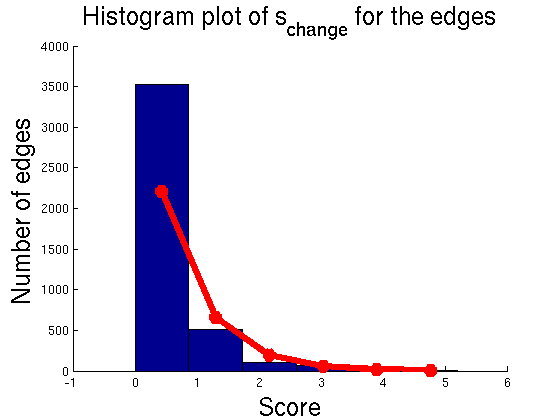
\includegraphics[scale=0.5]{results/change_hist} \\
b. &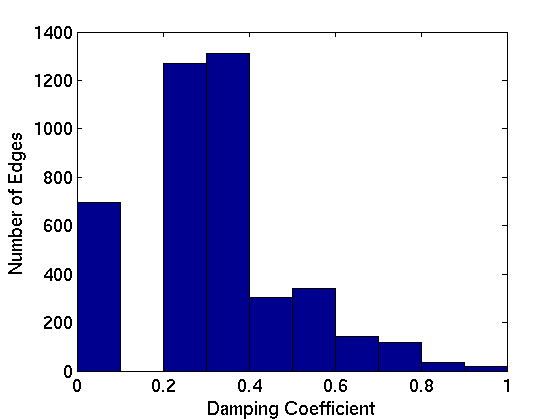
\includegraphics[scale=0.5]{results/strain_hist}  
  \end{tabular}
  \caption{This figure presents  histograms characterizing the change
    in the interaction strengths over all edges when the inference is
    done over JOINT (both strain) in Experiment~2 (a). We also show
    the histogram of the damping coefficients for the edges in the
    perturbed strain in Experiment 2 (b). It is important to note that the damping
    coefficients are dependent on the network topology.}
  \label{fig:hist-score}
\end{figure}


%Figure~\ref{fig:hist-score} (a) shows the histogram for the
%change score and the fitted exponential distribution. This is used to
%identify the interactions which have a high degree of change as
%described in \ref{sec:ident-crit-inter}. Figure~\ref{fig:hist-score}
%(b) shows the histogram of the strain damping coefficients obtained
%for the MUT strain which has the gene, YLR403W, deleted to
%glucose. 

%Figure~\ref{fig:plot-evol-1} shows the critical iteractions identified
%as described in \ref{sec:ident-crit-inter}, for the REF and MUT
%strains separately and then JOINT which does inference by combining
%the expression levels for both strains using the strain damping
%model. 

\begin{table}[htp]
  \centering
  \begin{tabular}{|l|l|}
\hline 
\textbf{MIPS ID} & \textbf{Description of functional categories} \\
\hline
\update{01.03.01} & purin nucleotide/nucleoside/nucleobase metabolism \\
10 & cell cycle and DNA processing \\
10.01.09 & DNA restriction or modification \\
10.03.01 & mitotic cell cycle and cell cycle control \\
\update{11.04.02} & tRNA processing \\
\update{12} & protein synthesis \\
\update{12.01.01} & ribosomal proteins \\
14.13.01 & cytoplasmic and nuclear protein degradation \\
\multirow{2}{*}{16} & protein with binding function or cofactor
 \\
& requirement (structural or catalytic) \\
16.02 & peptide binding \\
16.03.03&  RNA binding \\
16.21 & complex cofactor/cosubstrate/vitamine binding \\
\update{20.01.10} & protein transport \\
\update{20.01.15} & electron transport \\
\update{20.01.27} & drug/toxin transport \\
\update{20.09.03} & peroxisomal transport \\
\update{20.09.07} & vesicular transport (Golgi network, etc.) \\
\update{30} & cellular communication/signal transduction mechanism \\
\update{32.01.04} & pH stress response \\
32.05.05 & virulence, disease factors \\
32.07 & detoxification \\
32.07.07 & oxygen and radical detoxification \\
34.07.02 & cell-matrix adhesion \\
40.01.03 & directional cell growth (morphogenesis) \\
40.01.05 & growth regulators / regulation of cell size \\
42.04.03 & actin cytoskeleton \\
\hline
  \end{tabular}
 \caption{Description of the functional categories corresponding to the MIPS IDs identified in Table~\ref{tab:exp2-cat}.}
  \label{tab:exp2-list}
\end{table}
 
\begin{table}
  \centering
  \begin{tabular}{|c|c|c|}
    \hline
    \textbf{REF} & \textbf{MUT} & \textbf{JOINT} \\
\hline
\update{32.01.04} & \update{32.01.04} & \update{32.01.04} \\ 
\update{20.09.03} & \update{20.09.03} & \update{20.09.03} \\ 
10 &  16.21 & 16.21 \\ 
16.21 & 32.05.05 & \update{11.04.02} \\ 
\update{11.04.02} & 10 & 10 \\ 
32.05.05 & \update{11.04.02} & \update{12} \\ 
\update{20.01.27} & 40.01.05 & 32.05.05 \\ 
\update{30} & \update{30} & \update{30} \\ 
16.03.03 & 10.01.09 & 16.03.03 \\ 
\update{20.09.07} & 10.03.01 & 32.07 \\ 
\update{12} & 14.13.01 & \update{20.09.07} \\ 
32.07 & \update{20.01.10} & 40.01.03 \\ 
\update{20.01.15} & 16.03.03 & \update{20.01.27} \\ 
42.04.05 & \update{20.09.07} & 10.01.09 \\ 
34.07.02 & 42.04.03 & 34.07.02 \\ 
10.03.01 & 16 & 32.07.07 \\ 
40.01.03 & 34.07.02 & 16.02 \\ 
10.01.09 & \update{12.01.01} & 42.04.05 \\ 
42.29 & \update{01.03.01} & 42.29 \\ 
\hline  
\end{tabular}
  \caption{This table shows the list of functional categories which show
    the maximum amount of variation in time for the strains: (a) REF
    (b) MUT and (c) in both strains combined, using the damping model. The description for the categories can be found
  in Table~\ref{tab:exp2-list}. The categories indicated in blue are
  those which are known to have been enriched in the original
  dataset~\citep{Cipollina2008}.}
  \label{tab:exp2-cat}
\end{table}


% \begin{figure*}
%   \centering
%  \label{fig:plot-evol-1}
%   \begin{tabular}{lccc}
% T &  a.  & b. & c. \\
% t=0& 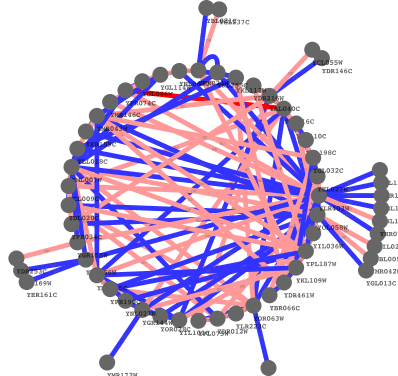
\includegraphics[scale=0.28]{results/ref/t1.png}
% & 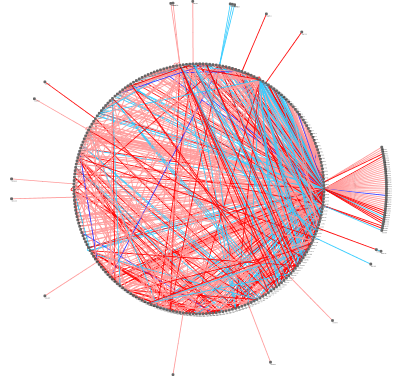
\includegraphics[scale=0.28]{results/mut/t1.png} & 
% 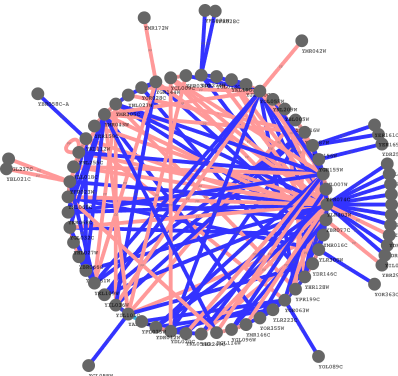
\includegraphics[scale=0.28]{results/joint/t1.png} \\
%  t=5  &   
\includegraphics[scale=0.28]{results/ref/t2.png}
%   &     
\includegraphics[scale=0.28]{results/mut/t2.png}
%  &     
\includegraphics[scale=0.28]{results/joint/t2.png} \\
%  t=10 &       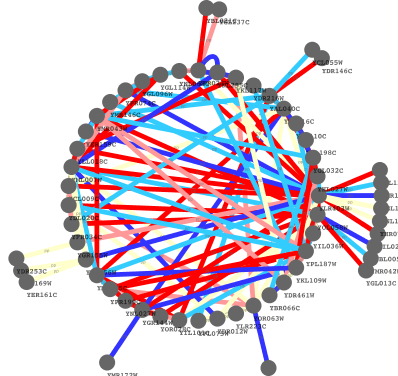
\includegraphics[scale=0.28]{results/ref/t3.png}
%        &     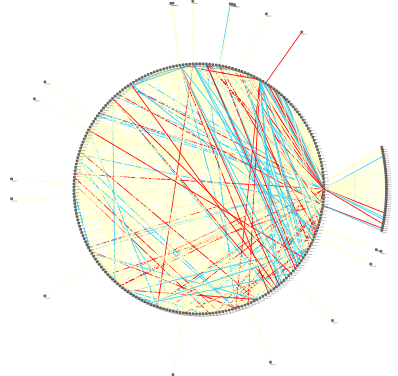
\includegraphics[scale=0.28]{results/mut/t3.png}
%        &     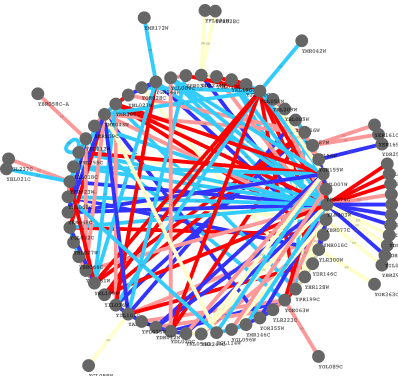
\includegraphics[scale=0.28]{results/joint/t3.png}  \\ 
%   t=30 &  
\includegraphics[scale=0.28]{results/ref/t4.png}
%      &      
\includegraphics[scale=0.28]{results/mut/t4.png}
%      &  
\includegraphics[scale=0.28]{results/joint/t4.png} \\
%  t=60 &   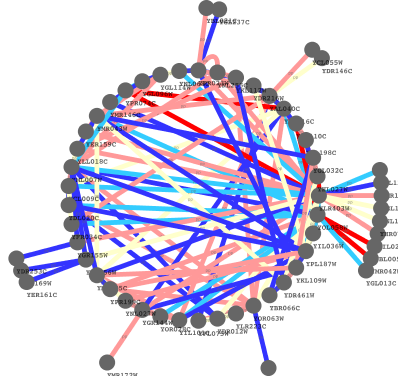
\includegraphics[scale=0.28]{results/ref/t5.png}
% &     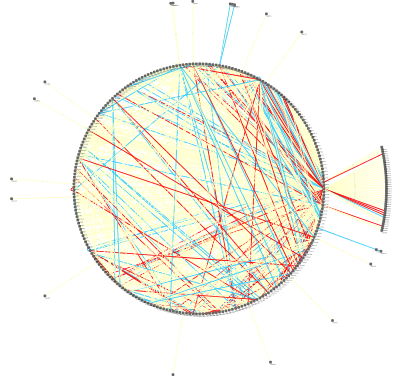
\includegraphics[scale=0.28]{results/mut/t5.png}
% &     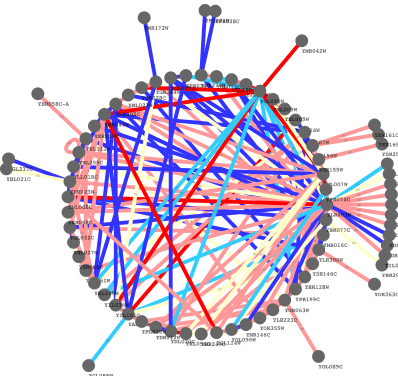
\includegraphics[scale=0.28]{results/joint/t5.png} \\
% t=120 &    
\includegraphics[scale=0.28]{results/ref/t6.png} 
% &     
\includegraphics[scale=0.28]{results/mut/t6.png} 
% &     
\includegraphics[scale=0.28]{results/joint/t6.png} 
%   \end{tabular}
%   \caption{Dynamics of temporal interactions between genes in REF (a),
%     MUT (b) and in both strains combined, using the damping model (c)
%     for Experiment 2. All the genes identified to be significantly
%     changed \citep{Cipollina2008} were combined into one network. The
%     color of the edges in the network indicates the interaction
%     strength, which was classified as strong repressing (red), low
%     repressing (pink), no effect (yellow), low inducing (light blue)
%     and strong inducing (dark blue). The time stamps (in minutes) are
%     indicated below each network. }
% \end{figure*}

\begin{figure*}
  \centering
 \label{fig:plot-evol-1}
  \begin{tabular}{lcccccc}
  a.  & 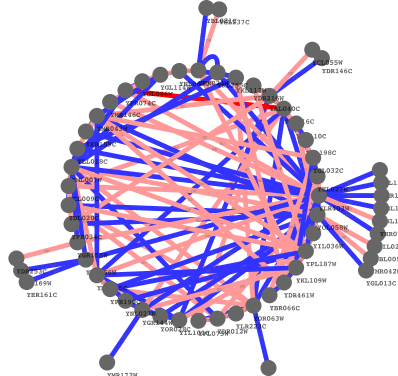
\includegraphics[scale=0.15]{results/ref/t1.png}
    &     
\includegraphics[scale=0.15]{results/ref/t2.png}
    &     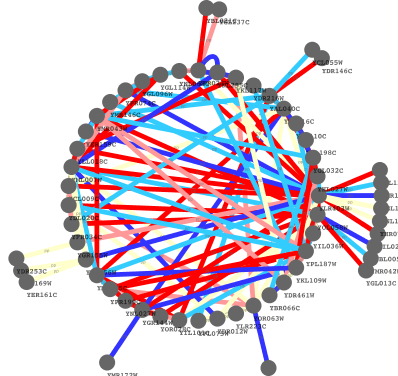
\includegraphics[scale=0.15]{results/ref/t3.png} 
&     
\includegraphics[scale=0.15]{results/ref/t4.png}
&     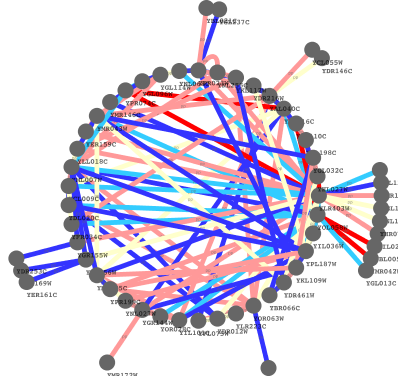
\includegraphics[scale=0.15]{results/ref/t5.png}
&     
\includegraphics[scale=0.15]{results/ref/t6.png} \\
  b.  &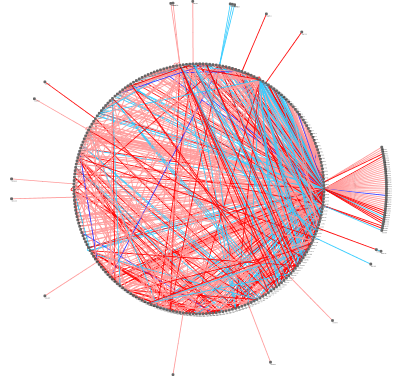
\includegraphics[scale=0.16]{results/mut/t1.png}
    &     
\includegraphics[scale=0.16]{results/mut/t2.png}
    &     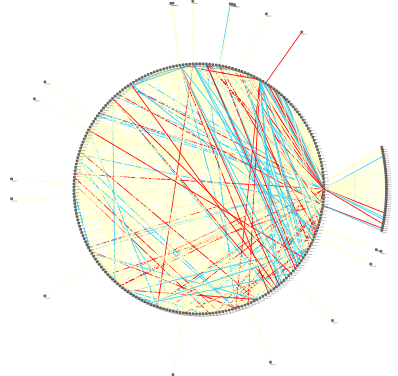
\includegraphics[scale=0.16]{results/mut/t3.png} 
&     
\includegraphics[scale=0.16]{results/mut/t4.png}
&     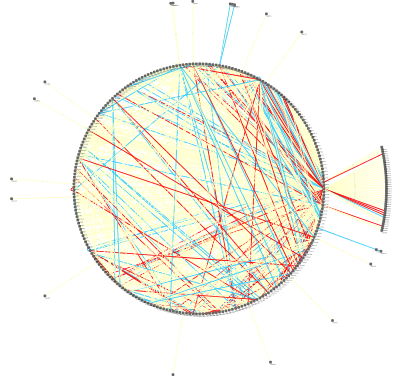
\includegraphics[scale=0.16]{results/mut/t5.png}
&     
\includegraphics[scale=0.16]{results/mut/t6.png} \\
 c.   & 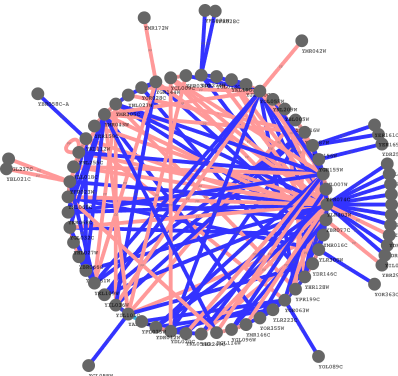
\includegraphics[scale=0.15]{results/joint/t1.png}
    &     
\includegraphics[scale=0.15]{results/joint/t2.png}
    &     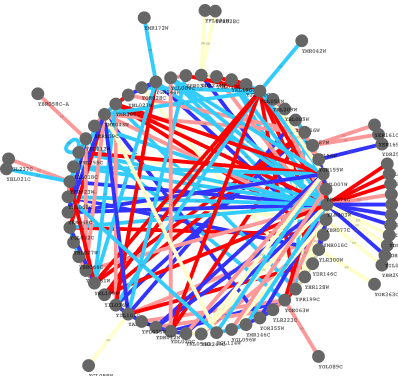
\includegraphics[scale=0.15]{results/joint/t3.png} 
&     
\includegraphics[scale=0.15]{results/joint/t4.png}
&     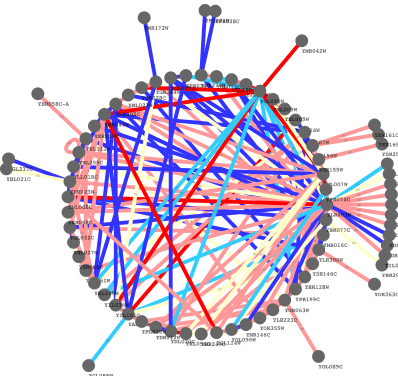
\includegraphics[scale=0.15]{results/joint/t5.png}
&     
\includegraphics[scale=0.15]{results/joint/t6.png} \\
&  t=0 & t=5 & t=10 & t=30 & t=60 & t=120
  \end{tabular}
  \caption{Dynamics of temporal interactions between genes in REF (a), MUT (b) and in both strains combined, using the damping model (c) for Experiment 2. All the genes identified to be significantly changed \citep{Cipollina2008} were combined into one network. The color of the edges in the network indicates the interaction strength, which was classified as strong repressing (red), low repressing (pink), no effect (yellow), low inducing (light blue) and strong inducing (dark blue). The time stamps (in minutes) are indicated below each network.}
\end{figure*}

\section{Conclusion}
\label{sec:conclusions}
There is a trade off between using more sophisticated conditional probability models $p(\mathbf{w}^{s}(t) |\mathbf{w}^{0}(t))$ involving more parameters to be learnt and the limited amount of experimental data. NETGEM is a systematic model that relates temporal changes in gene expression data to the dynamics of interactions in the context of a regulatory network. We believe that NETGEM achieves an optimal balance between model complexity and the data requirement, while allowing ample flexibility to adjust the parameters. The framework of the model will also inherently facilitate analyzing the effect of a perturbation in the network. For a given regulatory network and a gene expression data, NETGEM was able to identify time-sensitive interactions in the network and determine their strength. It was able to deduce most active functional categories that interacted. In addition to these, the NETGEM uses a damping feature that models the effect of a network perturbation by localizing more activity around the point of perturbation. These three novel features that NETGEM offers reflect its advantage over many other time-series models that have been developed recently. Of particular interest is its ability to capture abrupt changes in the interaction patterns. For example, NETGEM identified momentary arrest in ribosome biosynthesis during the transition in the nutrient that limits growth from glucose to ammonia (Experiment 1). We identified many actively interacting genes that were implicated to play an important role in the biological conditions from which we obtained the data. This lends the promise that new insights obtained from using NETGEM are also physiologically relevant. Given that the inputs to NETGEM are the topology of the network and temporal variation of the nodes, it is evident that this methodology has widespread applications in analyzing network dynamics, beyond biological systems.
\section{Acknowledgements}
GNV acknowledges funding from Chalmers Research Foundation and
  salary  from EC-funded project, UNICELLSYS. The authors also acknowledge Torbj\"orn Karfunkel for assistance with constructing the protein interaction network and discussion on the method.

%\bibliographystyle{bioinformatics}
%\bibliography{default}
\begin{thebibliography}{}

\bibitem[Androulakis {\em et~al.}, 2007]{Androulakis2007}
Androulakis, I.~P., Yang, E.  \& Almon, R.~R. (2007{\em{}}) Analysis of
  time-series gene expression data: methods, challenges, and opportunities.
\newblock {\em Annual Review of Biomedical Engineering, } {\bf 9} (1),
  205--228.

\bibitem[Bader {\em et~al.}, 2003]{Bader:2003:Nucleic-Acids-Res:12519993}
Bader, G.~D., Betel, D.  \& Hogue, C.~W. (2003{\em{}}) Bind: the biomolecular
  interaction network database.
\newblock {\em Nucleic acids research, } {\bf 31} (1), 248--250.

% \bibitem[Beal, 2003]{Beal03}
% Beal, M.~J. (2003{\em{}}).
% \newblock {\em Variational Algorithms for Approximate Bayesian Inference}.
% \newblock PhD thesis, Gatsby Computational Neuroscience Unit, University
%   College London.

\bibitem[Cipollina {\em et~al.}, 2008]{Cipollina2008}
Cipollina, C. {\em et~al.}  (2008{\em{}}) Saccharomyces cerevisiae SFP1: at the crossroads of central metabolism and ribosome biogenesis
\newblock {\em Microbiology, } {\bf 154} , 1686--1699.

\bibitem[Coughlan \& Shen, 2004]{Coughlan04}
James~M. Coughlan and Huiying Shen.
\newblock Shape matching with belief propagation: Using dynamic quantization to
  accommodate occlusion and clutter.
\newblock In {\em Generative-Model Based Vision workshop at CVPR}, 2004.

\bibitem[Dempster {\em et~al.}, 1977]{Dempster77em}
Dempster, A.~P., Laird, N.~M.  \& Rubin, D.~B. (1977{\em{}}) Maximum likelihood
  from incomplete data via the em algorithm.
\newblock {\em Journal of the Royal Statistical Society. Series B
  (Methodological), } {\bf 39} (1), 1--38.

\bibitem[Ernst \& Joseph, 2006]{Ernst06STEM}
Ernst, J. \& Joseph, Z.~B. (2006{\em{}}) Stem: a tool for the analysis of short
  time series gene expression data.
\newblock {\em BMC Bioinformatics, } {\bf 7} (1).

\bibitem[Farzadfard {\em et~al.}, 2010]{Farzadfard2010}
Farzadfard, F. {\em et~al.} (2010{\em{}})
  Metabolic and transcriptional dynamics during the transition from carbon
  limitation to nitrogen limitation in Saccharomyces cerevisiae.
\newblock {\em Genome Biology (in review)}.

\bibitem[Gavin {\em et~al.}, 2006]{Gavin2006}
Gavin, A.~C., {\em et~al.} (2006{\em{}}) Proteome survey reveals
  modularity of the yeast cell machinery.
\newblock {\em Nature, } {\bf 440}, 631--636.

\bibitem[Gavin {\em et~al.}, 2002]{Gavin2002}
Gavin, A.~C., {\em et~al.} (2002{\em{}}) Functional
  organization of the yeast proteome by systematic analysis of protein
  complexes.
\newblock {\em Nature, } {\bf 415}, 141--147.

\bibitem[Gelman {\em et~al.}, 2003]{Gelman03bayesian}
Gelman, A. {\em et~al.} (2003{\em{}}) {\em
  Bayesian Data Analysis, Second Edition (Texts in Statistical Science)}.
\newblock 2 edition,, Chapman \& Hall/CRC.

\bibitem[Gentleman {\em et~al.}, 2004]{Gentleman2004}
Gentleman, R.~C. {\em et~al.} (2004{\em{}}) Bioconductor: open software development for
  computational biology and bioinformatics.
\newblock {\em Genome Biology, } {\bf 5} (10), R80.

%\bibitem[Ghahramani \& Jordan, 1997]{DBLP:journals/ml/GhahramaniJ97}
%Ghahramani, Z. \& Jordan, M.~I. (1997{\em{}}) Factorial hidden markov models.
%\newblock {\em Machine Learning, } {\bf 29} (2-3), 245--273.

\bibitem[Glass \& Kaplan., 1993]{Glass1993}
Glass, L. \& Kaplan., D. (1993{\em{}}) Time series analysis of complex dynamics
  in physiology and medicine.
\newblock {\em Med Prog Technol, } {\bf 19}, 115--128.

\bibitem[Ho {\em et~al.}, 2002]{Ho2002}
Ho, Y. {\em et~al.} (2002{\em{}}) Systematic
  identification of protein complexes in saccharomyces cerevisiae by mass
  spectrometry.
\newblock {\em Nature, } {\bf 415}, 180--3.

\bibitem[Horn \& Johnson, 1990]{Horn90}
Horn, R.~A. \& Johnson, C.~R. (1990{\em{}}) {\em Matrix Analysis}.
\newblock {Cambridge University Press}.

\bibitem[Ito {\em et~al.}, 2001]{Ito2001}
Ito, T. {\em et~al.}
  (2001{\em{}}) A comprehensive two-hybrid analysis to explore the yeast
  protein interactome.
\newblock {\em PNAS, } {\bf 98}, 4569--74.

\bibitem[Krogan {\em et~al.}, 2006]{Krogan2006}
Krogan, N.~J. {\em et~al.} (2006{\em{}}) Global landscape of protein
  complexes in the yeast saccharomyces cerevisiae.
\newblock {\em Nature, } {\bf 440}, 637--43.

\bibitem[Leek {\em et~al.}, 2006]{Leek06EDGE}
Leek, J.~T. {\em et~al.} (2006{\em{}}) {EDGE:
  extraction and analysis of differential gene expression}.
\newblock {\em Bioinformatics, } {\bf 22} (4), 507--508.

% \bibitem[MacDonald \& Zucchini, 1997]{MacDonald1997}
% MacDonald, I.~L. \& Zucchini, W. (1997{\em{}}) {\em Hidden Markov and other
%   models for discrete-valued time series}.
% \newblock 1 edition,, Chapman \& Hall, London; New York.

% \bibitem[Mclachlan \& Krishnan, 1996]{Mclachlan97embook}
% Mclachlan, G.~J. \& Krishnan, T. (1996{\em{}}) {\em The EM Algorithm and
%   Extensions}.
% \newblock 1 edition,, Wiley-Interscience.

\bibitem[Mewes {\em et~al.}, 2007]{Mewes2007}
Mewes, H.~W. {\em et~al.} (2007{\em{}}) {MIPS: analysis and annotation of genome information in
  2007}.
\newblock {\em Nucleic Acids Res, } {\bf 36}.

\bibitem[Mewes {\em et~al.}, 2002]{MIPS}
Mewes, H.~W. {\em et~al.} (2002{\em{}}) Mips: a database for genomes and protein sequences.
\newblock {\em Nucleic acids research, } {\bf 30} (1), 31--34.

\bibitem[Petranovic \& Vemuri, 2009]{Petranovic2009}
Petranovic, D. \& Vemuri, G.~N. (2009{\em{}}) Impact of yeast systems biology
  on industrial biotechnology.
\newblock {\em J Biotechnol, } {\bf 144} (3), 204--11.

\bibitem[Rabiner, 1989]{Rabiner89hmm}
Rabiner, L.~R. (1989{\em{}}) A tutorial on hidden markov models and selected
  applications in speech recognition.
\newblock {\em Proceedings of the IEEE, } {\bf 77} (2), 257--286.

\bibitem[Ramoni {\em et~al.}, 2002]{Ramoni02cluster}
Ramoni, M.~F. {\em et~al.} (2002{\em{}}) Cluster analysis
  of gene expression dynamics.
\newblock {\em Proc Natl Acad Sci U S A, } {\bf 99} (14), 9121--9126.

\bibitem[Schliep {\em et~al.}, 2003]{DBLP:conf/ismb/SchliepSS03}
Schliep, A. {\em et~al.} (2003{\em{}}) Using hidden
  markov models to analyze gene expression time course data.
\newblock In {\em ISMB (Supplement of Bioinformatics)} pp. 255--263.

\bibitem[Shannon {\em et~al.}, 2003]{Shannon2003}
Shannon, P. {\em et~al.} (2003{\em{}}) Cytoscape: a software
environment for integrated models of biomolecular interaction networks 
\newblock In {\em Genome Research}  {\bf 13} (11), pp. 2498 --2504.

\bibitem[Song {\em et~al.}, 2009]{Song09KELLER}
Song, L., Kolar, M.  \& Xing, E.~P. (2009{\em{}}) Keller: estimating
  time-varying interactions between genes.
\newblock {\em Bioinformatics, } {\bf 25} (12).

\bibitem[Stark {\em et~al.}, 2006]{citeulike:814974}
Stark, C. {\em et~al.} (2006{\em{}}) Biogrid: a general repository for interaction
  datasets.
\newblock {\em Nucleic Acids Res, } {\bf 34} (Database issue).

\bibitem[Stigler {\em et~al.}, 2007]{Stigler2007}
Stigler, B. {\em et~al.} (2007{\em{}})
  Reverse engineering of dynamic networks.
\newblock {\em Ann N Y Acad Sci, } {\bf 1115}, 168--77.

\bibitem[Uetz {\em et~al.}, 2000]{Uetz2000}
Uetz, P. {\em et~al.} (2000{\em{}}) A
  comprehensive analysis of protein-protein interactions in saccharomyces
  cerevisiae. :.
\newblock {\em Nature, } {\bf 403}, 623--7.

\bibitem[Xenarios {\em et~al.}, 2000]{citeulike:226627}
Xenarios, I. {\em et~al.} (2000{\em{}}) Dip: the database of interacting proteins.
\newblock {\em Nucl. Acids Res., } {\bf 28} (1), 289--291.

\bibitem[Yoneya \& Mamitsuka, 2007]{Yoneya2007}
Yoneya, T. \& Mamitsuka, H. (2007{\em{}}) A hidden markov model-based approach
  for identifying timing differences in gene expression under different
  experimental factors.
\newblock {\em Bioinformatics, } {\bf 23} (7).

\bibitem[Zanzoni, 2002]{citeulike:3733950}
Zanzoni, A. (2002{\em{}}) Mint: a molecular interaction database.
\newblock {\em FEBS Letters, } {\bf 513} (1), 135--140.
\end{thebibliography}

\end{document}